\documentclass{article}

\usepackage{amsmath}
\usepackage{graphicx}
\usepackage{epstopdf}
\usepackage{subfigure}
\usepackage{fullpage}

\author{Taylor Southwick and Tyler Southwick}
\title{Multiagent Lab}
\begin{document}
\maketitle

\section{Finite State Machine}
The decoy was set into a path using potential fields that would draw it north and then draw it south when it reached each of the points.  This point was set to be at a location closer to the guards than the sniper, but far enough that the bullets from the guards would take some time to get there.  The decoy remained on this path, alternating between the two points, indefinitely once the position was assumed.

Once the sniper made its way to the presposition, it waited for the decoy to assume its alternative position of going north and south.  Once this has happened, the sniper then makes its way to a point farther away from the guards than the decoy, but close enough that it can shoot.  At this point, he systematically shoots at each enemy.  For each enemy, it adjusts its angle to have a straight line shot toward the enemy, then shoots.  If this fails, it continues until it has succeed.  

At this point, the sniper goes for the flag, being attracted to it with a potential field.  Upon capturing the flag, a search path is found to the goal.  The same procedure as described above was used to guide the sniper back to the goal with the retrieved flag.

\section{Use of Potential Fields}

\section{Search Path}
In order to search the world, we needed to discretize it.  This was done by building off of the occgrid concept, but creating it ourselves.  This occgrid could have an arbitrary resolution, and would populate the world with information about obstacles (enemies can be added if needed).  We found that adding the enemy was essentially of no use, since they would block the path to the points and therefore cause it to be impossible to find a route.  This occgrid is shown in Fig.~\ref{fig:occgrid}

We calculated the search path by using the A* algorithm.  The starting point was the location of the individual tank each time, with the ending point different if the tank was a sniper or a decoy.  This ending point, termed the \emph{preposition} point, was situated so that it would be far enough from the enemies that their shots would not affect our tanks.  The sniper had a point located close to the opening of the maze, while the decoy had a point a bit north-northeast of the sniper. To see the search path found to the preposition points and the flag, see Fig.~\ref{fig:searchpaths}.
\begin{figure}[h!]
	\subfigure[Decoy]{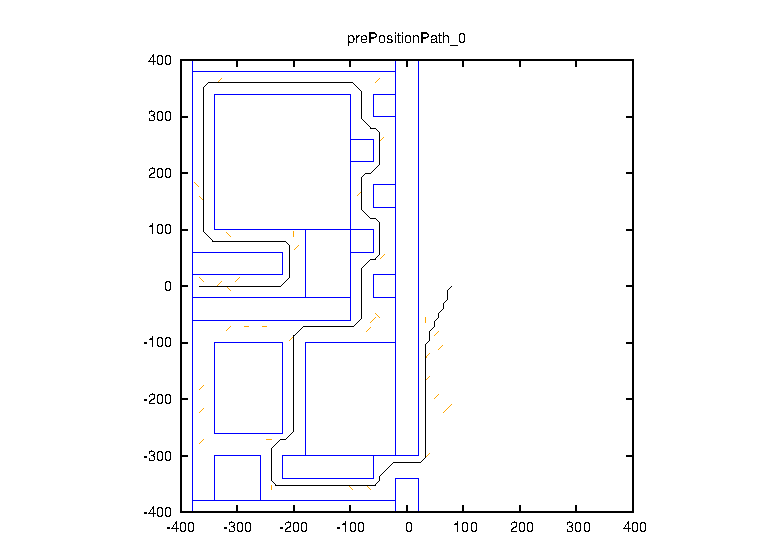
\includegraphics[width=.30\textwidth]{graphics/prePosition_0}}
	\subfigure[Sniper]{\includegraphics[width=.30\textwidth]{graphics/prePosition_1}}
	\subfigure[Sniper w/ Flag]{\includegraphics[width=.30\textwidth]{graphics/returnHome_1}}
	\caption{Search paths generated by A*}
	\label{fig:searchpaths}
\end{figure}

\section{Movement along Search path}
The path gave the optimal route to these points, but the tanks can only be moved by manipulating the angular and forward velocities.  In order to follow the search path, a series of potential fields were created.  We found that if we were to use potential fields for the entire search path, there would be much computation that would do nothing, and it would adversely affect the resultant vectors.  So, in order to alleviate this, we decided to use a subset of the points.  This subset was defined based off of the node closest to the current point of the tank.  The specified number of nodes were skipped (which, for the resolution our occgrid was at turned out to be 3), and then, for the occgrid we used, 7 points were used to create the potential fields.  
\begin{figure}[h!tb]
	\subfigure[Decoy]{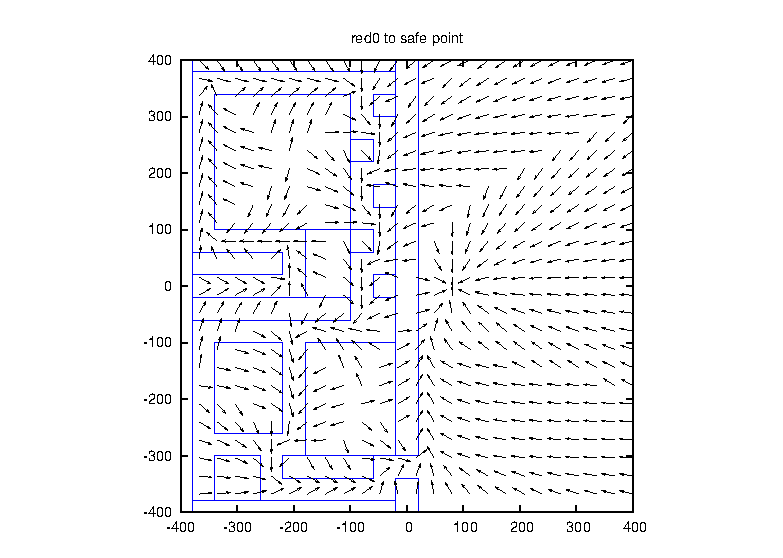
\includegraphics[width=.30\textwidth]{graphics/red0_safePoint}}
	\subfigure[Sniper]{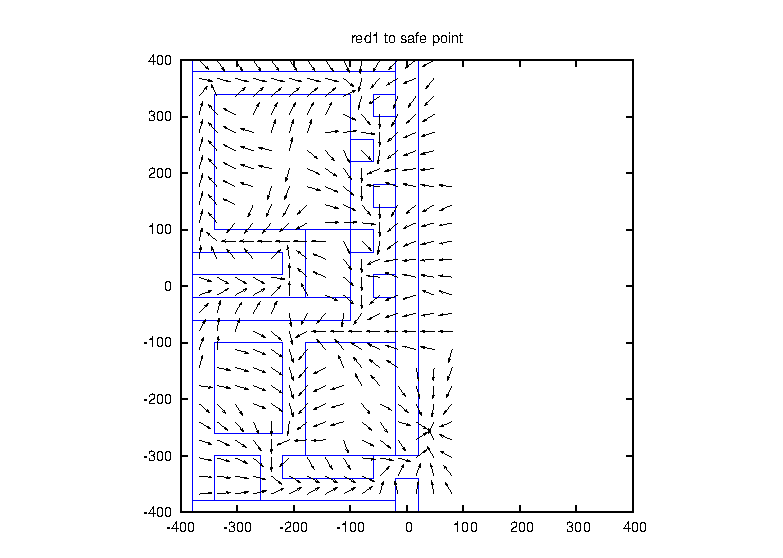
\includegraphics[width=.30\textwidth]{graphics/red1_safePoint}}
	\subfigure[Sniper w/ Flag]{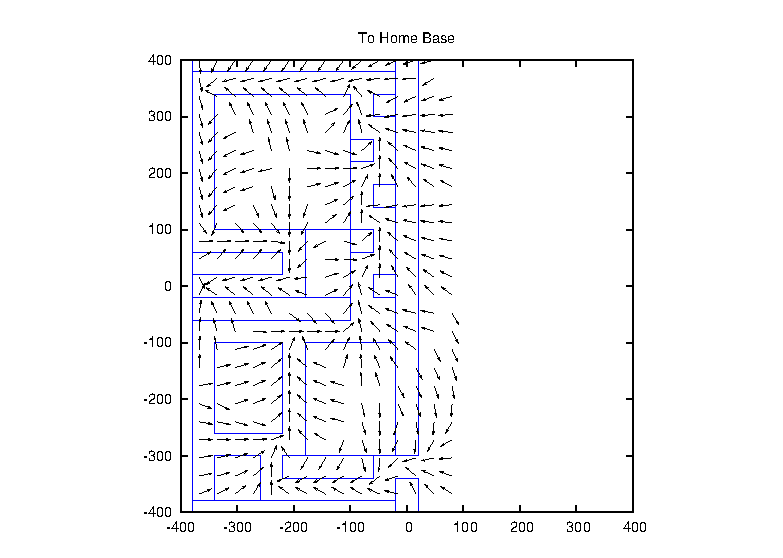
\includegraphics[width=.30\textwidth]{graphics/toHomeBase}}
	\caption{Potential field of Search Paths}
\end{figure}

As an example, consider Fig.~\ref{fig:graph_pf_generator}.  Since the tank is directed with a PD controller, often the position is not as intended.  The dotted line indicates the closest node in the search path.  If we were to use a PF to attract the tank to there, the result would be either slow movement or backtracking.  For the same reason, the next point is skipped.  Due to the resolution of this occgrid, only one node is skipped, followed by the three black nodes that are used to generate attractive potential fields.

\begin{figure}[h!tb]
	\label{fig:graph_pf_generator}
	\begin{center}
	\includegraphics[width=.4\textwidth,page=1]{graphics/drawing}
	\end{center}
	\caption{Graphical depiction of how potential fields were generated}
\end{figure}

\section{Future Improvements}

\section{Code Demonstration}
We demonstrated our code to Daniel Brown and Ryan Hintze. While watching theirs, we saw a difference in how the search path was followed.  Theirs would pick a point and go towards it, compared to the potential fields that ours used.  Ours seems to make a much smoother path, especially when it came to the jagged part of the maze. Theirs maneuvered the maze and had no issue killing the guards, collecting the flag, and returning home.

Ours took a couple of tries to finish, since our decoy was not following a path that could evade the puppyguards.  Once that was fixed, it went through all right and accomplished the goal, quicker than theirs did.

\newpage

\begin{figure}
	\begin{center}
	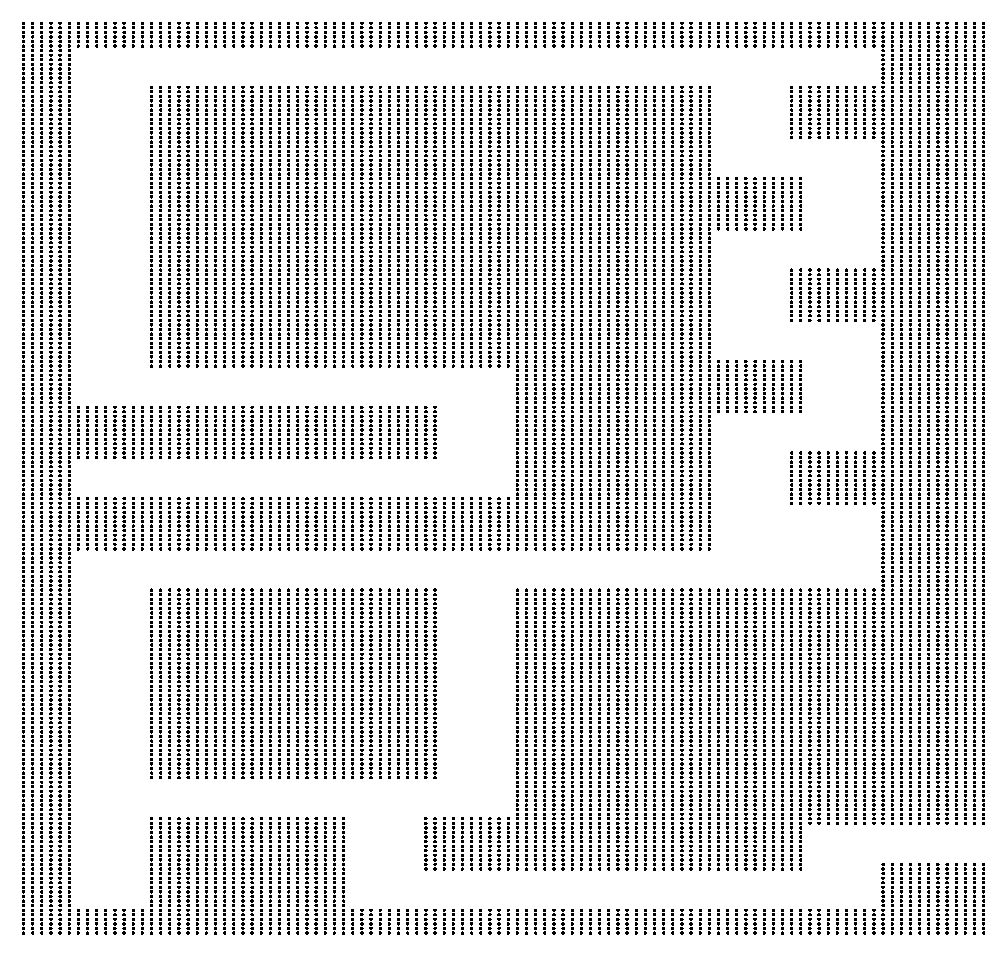
\includegraphics[width=\textwidth]{graphics/world.eps}
	\end{center}
	\caption{Representation of \emph{occgrid}}
	\label{fig:occgrid}
\end{figure}
\end{document}
